\documentclass[11pt]{article}
\usepackage{geometry} % Pour passer au format A4
\geometry{hmargin=1cm, vmargin=1cm} % 

% Page et encodage
\usepackage[T1]{fontenc} % Use 8-bit encoding that has 256 glyphs
\usepackage[english,french]{babel} % Français et anglais
\usepackage[utf8]{inputenc} 

\usepackage{lmodern}
\setlength\parindent{0pt}

% Graphiques
\usepackage{graphicx,float,grffile,hyperref}

% Maths et divers
\usepackage{amsmath,amsfonts,amssymb,amsthm,verbatim}
\usepackage{multicol,enumitem,url,eurosym,gensymb}

% Sections
\usepackage{sectsty} % Allows customizing section commands
\allsectionsfont{\centering \normalfont\scshape}

% Tête et pied de page

\usepackage{fancyhdr} 
\pagestyle{fancyplain} 

\fancyhead{} % No page header
\fancyfoot{}

\renewcommand{\headrulewidth}{0pt} % Remove header underlines
\renewcommand{\footrulewidth}{0pt} % Remove footer underlines

\newcommand{\horrule}[1]{\rule{\linewidth}{#1}} % Create horizontal rule command with 1 argument of height

\renewcommand{\labelitemi}{$\bullet$}
\renewcommand{\labelitemii}{$\circ$}

%----------------------------------------------------------------------------------------
%   Début du document
%----------------------------------------------------------------------------------------

\begin{document}

\setlength{\columnseprule}{1pt}

\section*{1 - Équations}

Un équation est un calcul à trou. On cherche un nombre dans un calcul et pas seulement un résultat. 

\subsection*{a - Le petit prince}

\textbf{Le Petit Prince} est un court roman très connu écrit par Antoine de Saint-Exupéry. C'est une œuvre poétique et philosophique qui prend l'apparence d'un conte pour enfants. 

On suit un aviateur qui tombe en panne et se pose en catastrophe dans le désert du Sahara. Il n’arrive pas à réparer son avion. Le lendemain, il est réveillé par un petit personnage qui lui demande : « S'il vous plaît… dessine-moi un mouton ! » 

\begin{figure}[H]
        \centering
        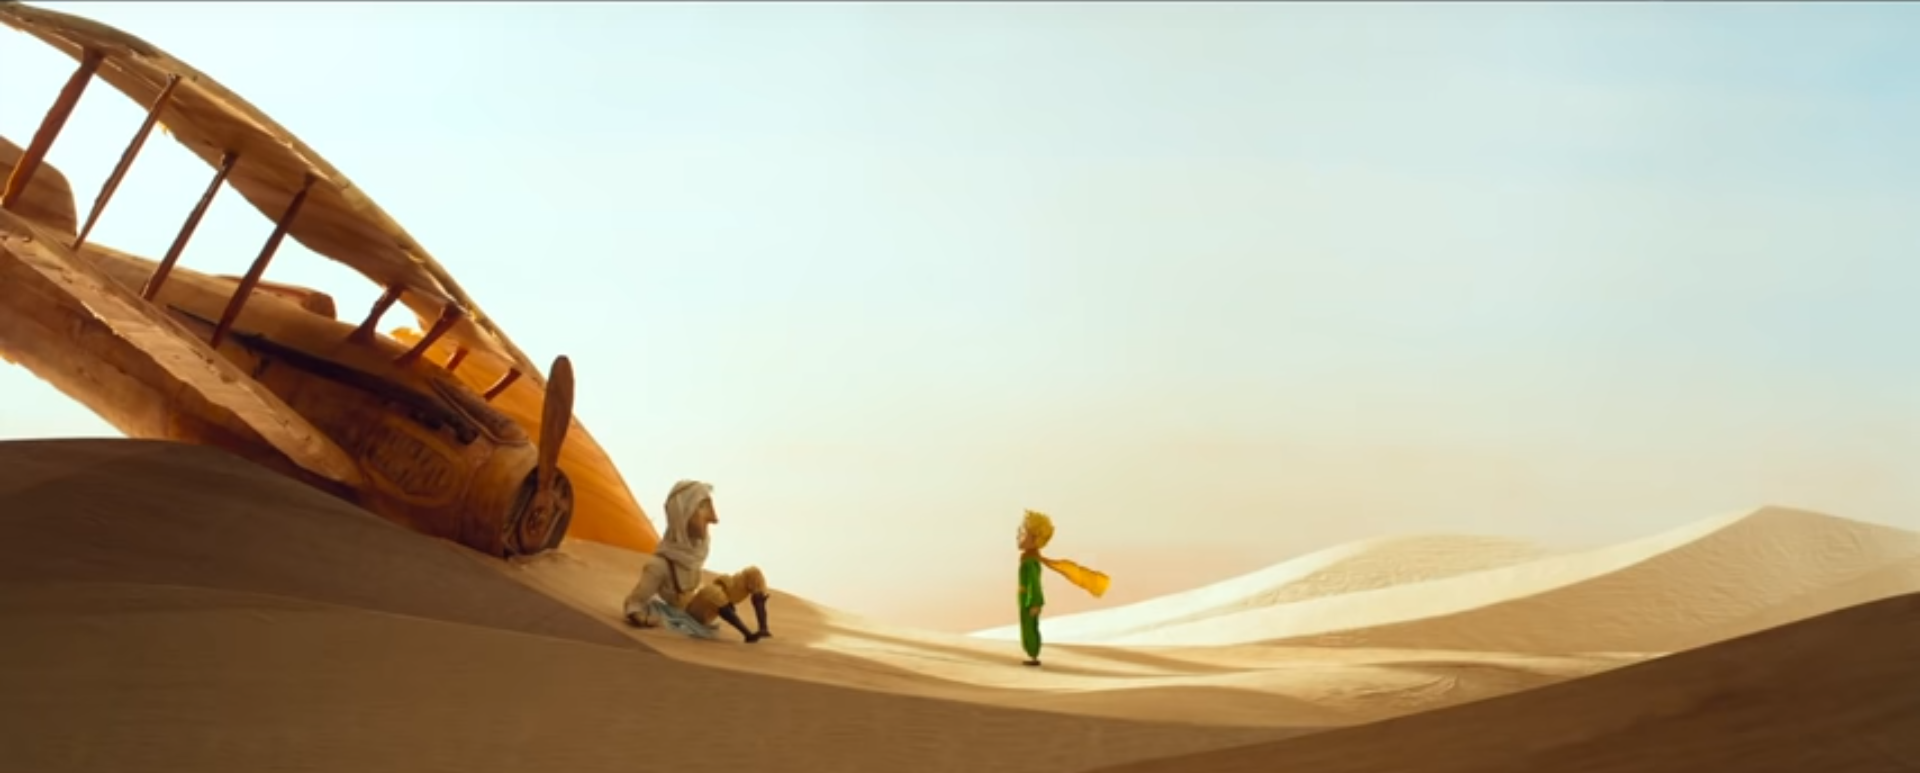
\includegraphics[width=0.5\linewidth]{3x11-equations/pp.png}
\end{figure}
\begin{center}
    \href{https://www.youtube.com/watch?v=JOWw5OaaZf8}{Youtube - Le petit prince} 
\end{center}


\textit{(Extrait du Petit Prince...)}

\begin{multicols}{2}
  \og S'il vous plaît… dessine-moi un mouton ! \fg \\
  Alors j'ai dessiné.
  
  \begin{figure}[H]
        \centering
        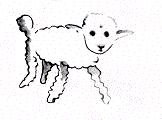
\includegraphics[width=0.3\linewidth]{3x11-equations/dm-mouton2.png}
  \end{figure}

  Il regarda attentivement, puis: \\
  - Non! Celui-là est déjà très malade. Fais-en un autre. \\
  Je dessinai:

  \begin{figure}[H]
        \centering
        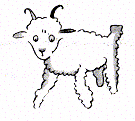
\includegraphics[width=0.3\linewidth]{3x11-equations/dm-mouton1.png}
  \end{figure}

  Mon ami sourit gentiment, avec indulgence: \\
  - Tu vois bien... ce n'est pas un mouton, c'est un bélier. Il a des cornes... \\
  Je refis donc encore mon dessin:

  \begin{figure}[H]
        \centering
        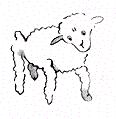
\includegraphics[width=0.3\linewidth]{3x11-equations/dm-mouton3.png}
  \end{figure}
  
  Mais il fut refusé, comme les précédents: \\
  - Celui-là est trop vieux. Je veux un mouton qui vive longtemps. \\
  Alors, faute de patience, comme j'avais hâte de commencer le démontage de mon moteur, je griffonnai ce dessin-ci.
  
  \begin{figure}[H]
        \centering
        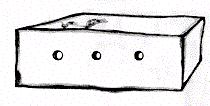
\includegraphics[width=0.5\linewidth]{3x11-equations/dm-mouton4.png}
  \end{figure}

  Et je lançai: \\
  - Ça c'est la caisse. Le mouton que tu veux est dedans. \\
  Mais je fus bien surpris de voir s'illuminer le visage de mon jeune juge: \\
  - \textbf{C'est tout à fait comme ça que je le voulais ! }
\end{multicols}

\newpage
\subsection*{b - du petit prince à la lettre $x$}

Il se passe la même chose en mathématiques. Quand l'intuition ne suffit pas, nous utilisons une \og boite à nombre \fg. \textbf{Une boite qui peut contenir le nombre que tu veux}. On appelle ce nombre $x$.

\vspace{1cm}
\centerline{\fontsize{102}{102} $x$}
\vspace{1cm}

\paragraph{Remarques : }Pourquoi est-il difficile d'avoir de l'intuition et de trouver un nombre qui \textit{marche} ? \\

Il existe une infinité de nombre et même plusieurs. Entre chaque nombre qu’on peut écrire, il y a un nombre qu’on ne peut pas écrire. Il existe plus de nombre en maths qu’il existe de mots. Il existe même des nombres qu’on ne sait pas écrire. C’est aussi pour ça qu’on a besoin d’\textbf{une lettre pour représenter tous les nombres qui existent.} \\

\subsection*{c - La rédaction et les étapes}

Dans ce chapitre, on va apprendre à \textbf{résoudre} des équations. Résoudre signifie trouver des solutions. On ne va pas se baser sur l’intuition. On va suivre \textbf{un protocole, une méthode}.\\

Il ne faut pas chercher la réponse puis la rédiger pour faire plaisir au professeur ou pour avoir une bonne note. il faut faire des étapes pour arriver à une réponse. Avec ce point de vue, cela peut sembler différent des rédactions en HG ou en Fr où l’on sait déjà un peu ce que l’on va dire et où on trouve des arguments qui vont avec notre idée principal. \\

\begin{center}\textbf{En mathématiques : Les étapes nous apportent une réponse.}\end{center}

On peut faire le parallèle avec la vie réelle et notre ressenti. On observe ce qui se passe puis on se fait une idée sans avoir avant des préjugés. 

\newpage
\section*{2 - Résoudre des équations}

Pour résoudre les équations au collège, on utilise la méthode d’\textbf{Al Khwarizmi}

\begin{figure}[H]
        \centering
        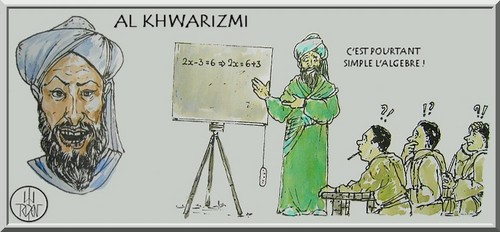
\includegraphics[width=0.5\linewidth]{3x11-equations/al.png}
\end{figure}
\begin{center}
    \href{https://www.maths-et-tiques.fr/index.php/histoire-des-maths/mathematiciens-celebres/al-khwarizmi}{Yvan Monka - Maths et Tiques}
\end{center}
\begin{multicols}{3}
\begin{enumerate}
    \item[1.] \textbf{Al-jabr} - devenu algèbre.\\
    $4x - 3 = 5$ \textit{(devient)} \newline
    $4x = 5 + 3$ \columnbreak
    \item[2.] \textbf{Al-muqabala} - La réduction. \\
    $4x = 3x + 9$ \textit{(devient)} \newline
    $4x - 3x = 9$ \columnbreak
    \item[3.] \textbf{Al-hatt} La division. \\
    $7x = 129$ \textit{(devient)} \newline
    $x - \dfrac{129}{7}$ 
\end{enumerate}
\end{multicols}

\begin{multicols}{2}
\paragraph{Remarques : } Le signe $=$ se lit dans les deux sens. \\
C’est aussi l’occasion de rappeler qu'on n’écrit pas : $10 + 2 = 12 * 2 = 24$. \columnbreak
    \begin{align*}
        2*6 &= 18  \\
        18 &= 2*6
    \end{align*}
    \begin{align*}        
        7 &= x + 3 \\
        x + 3 &= 7
    \end{align*}
\end{multicols}

Pour résoudre un équation de type collège, on utilise simplement ces trois méthodes l’une après l’autre :

\begin{center}
    \begin{enumerate}
        \item[1.] On met les nombres à droite, 
        \item[2.] on met mes x à gauche puis,  
        \item[3.] on divise par ce qui est devant x.
    \end{enumerate}
\end{center}

\paragraph{Deux exemples : } 
\begin{multicols}{2}
    \begin{align*}
        12x + 3 &= 14 \\
        12x &= 14 - 3 \\
        12x &= 11 \\
        x &= \dfrac{11}{12}
    \end{align*}
    \columnbreak
    \begin{align*}
        6x - 3 &= 4x - 4 \\
        6x &= 4x - 4 + 3 \\
        6x - 4x &= - 1 \\
        2x &= -1 \\
        x &= -\dfrac{1}{2}
    \end{align*}
\end{multicols}

\newpage

\paragraph{Remarques : }
\begin{itemize}
    \item Il faut essayer de se forger sa propre compréhension au fil des équations : 
    \begin{itemize}
        \item \og le + devient - \fg
        \item \og On passe le 2 de l’autre côté \fg
        \item \og On met une barre un peu plus loin avec écrit $-2$ pour dire qu’on appliqué -2 de chaque côté de l’équation \fg
        \item \og On annule : $x + 2 - 2 = 7 _ 2$ \fg
        \item \og…
    \end{itemize}

    \item Il existe plein de liens et de ressources pour essayer de comprendre à partir de quelqu’un d’autre et essayer d’aller plus loin.
    \begin{itemize}
        \item \href{https://www.youtube.com/watch?v=uV_EmbYu9_E}{Yvan Monka - \textit{(1 millions 200 mille vues)}}.
        \item \href{https://fr.khanacademy.org/math/be-2eme-secondaire2/x291d358f50a246d9:algebre-1/x291d358f50a246d9:equations/a/multi-step-equations-review}{Khan Academy}.
    \end{itemize}
\end{itemize}   

\begin{center}
    Pour réussir les équations, il faut s’entraîner. Dans ce chapitre, on va en résoudre \textbf{100}.
\end{center}

\newpage

\section*{3 - Les 100}

J’utilise le générateur : \href{https://gomaths.ch/print_alg_equ1d.php?nb_calcul=30&niveau=3}{gomaths.ch}.

\begin{multicols}{2}
\begin{enumerate}
    \item x + 3 = 0
    \item x + 10 = 12
    \item x + 2 = 4
    \item x - 6 = 16
    \item x - 10 = - 12
    \item 8 + x = 4
    \item -4 + x = -3
    \item 5 = x + 2
    \item 15 = 5 + x
    \item x + 10 = 10
    \item ...
\end{enumerate}
\end{multicols}
\newpage

\section*{4 - Et après ?}

Une fois les équations de bases maîtrisées, on peut rajouter des difficultés :  


\subsection*{a - Des petites choses pour aller plus loin}

\begin{enumerate}
    \item On met des nombres plus compliqués : $\pi$, $\sqrt{2}$, $\tfrac{4}{7}$ augmentent le risque d’erreurs de calcul mais ne change pas le protocole. 

    \item on rajoute des parenthèses. Il faut commencer par \textbf{distribuer}. 
    \begin{align*}
        2(x+3) &= 4x +1 \\
        2x + 6 &= 4x +1
    \end{align*}
          \item on passe aux équations produit : \\
        $(x+2)(x-4) = 0$  \\
       \textbf{Un produit est nul si l’un des facteurs est nul.}
       On regarde et résout :
    \begin{multicols}{2}
        \begin{align*}
            x+2 &= 0
            x &= -2
        \end{align*}
        \begin{align*}
            x-4 &= 0
            x &= 4
        \end{align*}
\end{multicols} 
		L’équation a deux solutions $-2$ et $4$.
    \end{enumerate}

Mais jusqu’à où peut-on compliquer une équation ? \\

Il est relativement simple d'écrire des équations. Il est difficile de toutes les résoudre. Il existe encore de nos jours des équations dont on ne connaît pas toutes les solutions. 

\newpage

\subsection*{b - Navier-Stokes}
Par exemple, le problème du millénaire sur l’équation de Navier-Stokes. On sait écrire l'équation... mais on ne sait pas la résoudre. Celui qui la trouvera empochera  $1 \, 000 \, 000 \$$ . Cela permettrait de connaître la météo de manière exacte. 


L'équation de Navier Stokes permet de prédire la météo, de comprendre les océans, les cours d'air et cours d'eau... On étudie la \textbf{turbulence}.

On sait écrire son équation : 

$$\rho \left({\dfrac {\partial e}{\partial t}}+\mathbf {V} \cdot \mathbf {\nabla } e\right)={\mathsf {P}}:\mathbf {\nabla } \mathbf {V} +\mathbf {\nabla } \cdot \mathbf {q} +\mathbf {\nabla } \cdot \mathbf {q} _{R}.$$

Mais on ne sait pas la résoudre.

  \begin{figure}[H]
        \centering
        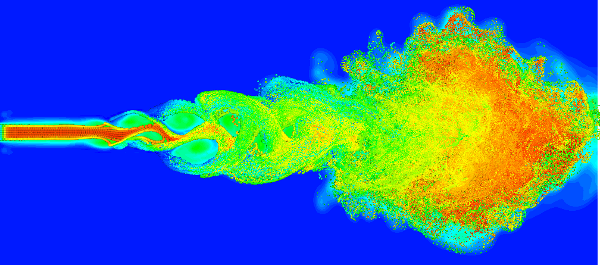
\includegraphics[width=0.6\linewidth]{3x11-equations/ns-1.png}
  \end{figure}

\begin{multicols}{2}

  \begin{figure}[H]
        \centering
        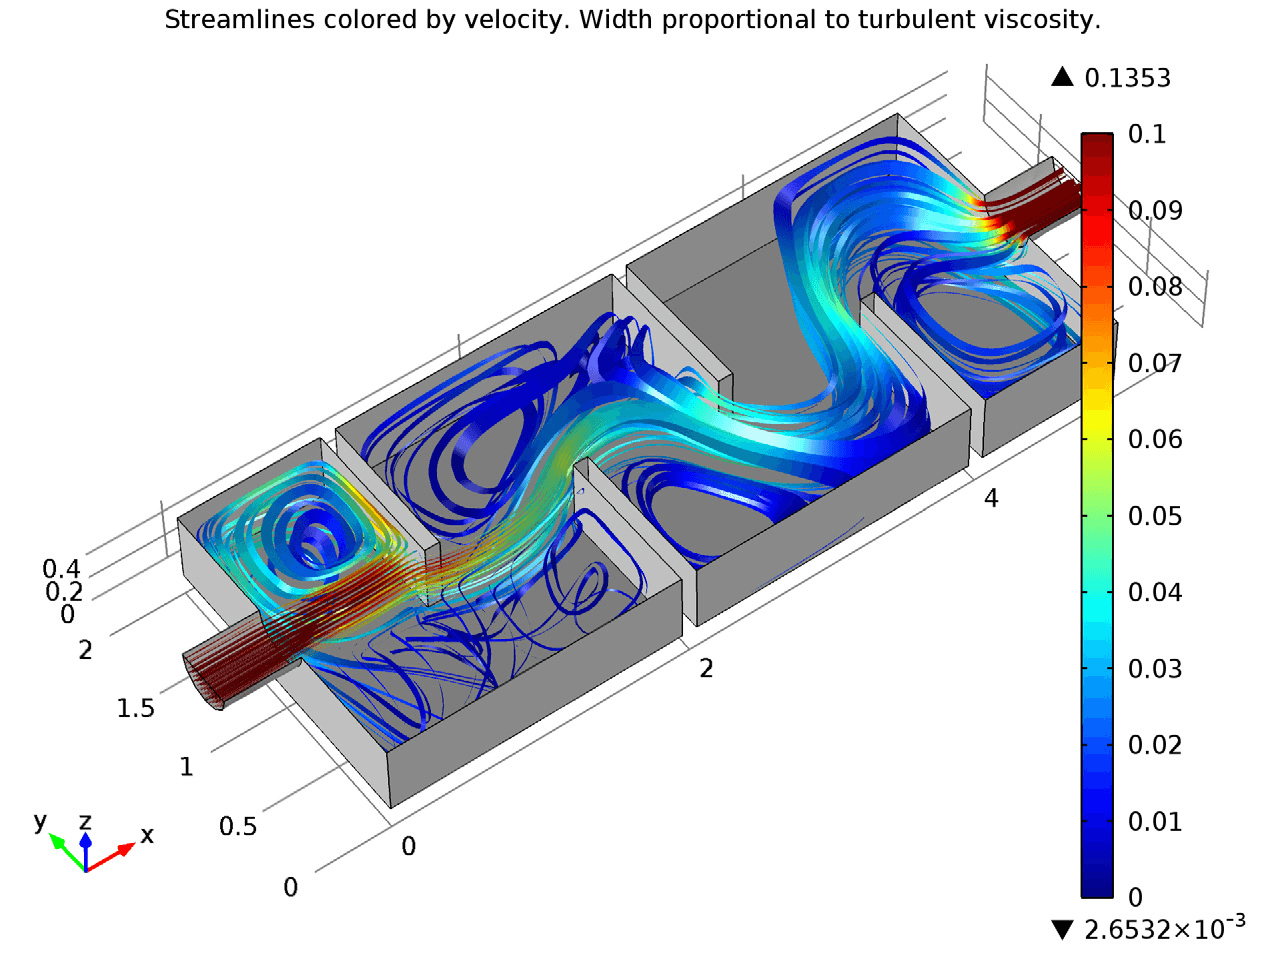
\includegraphics[width=0.8\linewidth]{3x11-equations/ns-2.png}
  \end{figure}
    \begin{figure}[H]
        \centering
        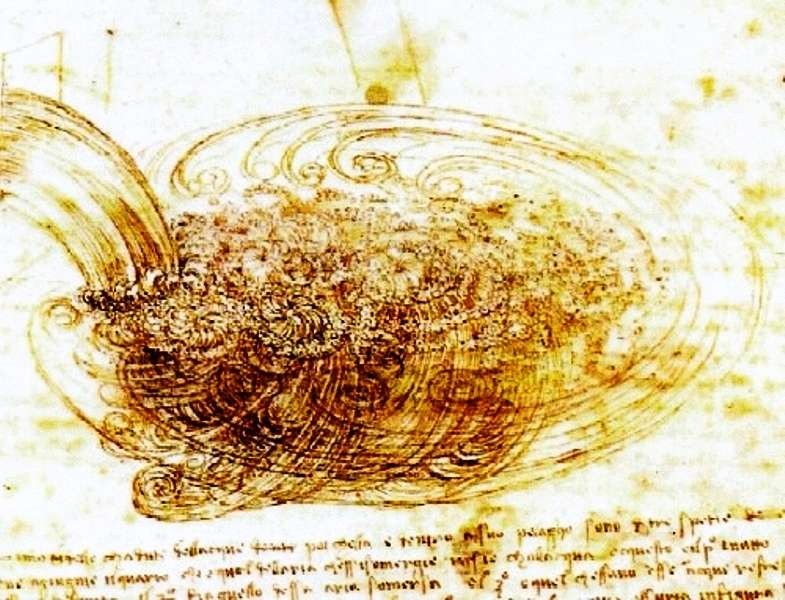
\includegraphics[width=0.8\linewidth]{3x11-equations/ns-3.png}
  \end{figure}

\end{multicols}

\begin{multicols}{2}

    \begin{figure}[H]
        \centering
        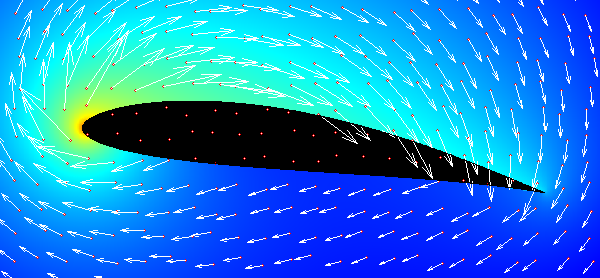
\includegraphics[width=0.8\linewidth]{3x11-equations/ns-4.png}
  \end{figure}

    \begin{figure}[H]
        \centering
        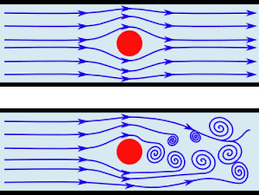
\includegraphics[width=0.8\linewidth]{3x11-equations/ns-5.png}
  \end{figure}
\end{multicols}



\end{document}
